\documentclass{article}\usepackage[]{graphicx}\usepackage[]{color}
%% maxwidth is the original width if it is less than linewidth
%% otherwise use linewidth (to make sure the graphics do not exceed the margin)
\makeatletter
\def\maxwidth{ %
  \ifdim\Gin@nat@width>\linewidth
    \linewidth
  \else
    \Gin@nat@width
  \fi
}
\makeatother

\definecolor{fgcolor}{rgb}{0.345, 0.345, 0.345}
\newcommand{\hlnum}[1]{\textcolor[rgb]{0.686,0.059,0.569}{#1}}%
\newcommand{\hlstr}[1]{\textcolor[rgb]{0.192,0.494,0.8}{#1}}%
\newcommand{\hlcom}[1]{\textcolor[rgb]{0.678,0.584,0.686}{\textit{#1}}}%
\newcommand{\hlopt}[1]{\textcolor[rgb]{0,0,0}{#1}}%
\newcommand{\hlstd}[1]{\textcolor[rgb]{0.345,0.345,0.345}{#1}}%
\newcommand{\hlkwa}[1]{\textcolor[rgb]{0.161,0.373,0.58}{\textbf{#1}}}%
\newcommand{\hlkwb}[1]{\textcolor[rgb]{0.69,0.353,0.396}{#1}}%
\newcommand{\hlkwc}[1]{\textcolor[rgb]{0.333,0.667,0.333}{#1}}%
\newcommand{\hlkwd}[1]{\textcolor[rgb]{0.737,0.353,0.396}{\textbf{#1}}}%
\let\hlipl\hlkwb

\usepackage{framed}
\makeatletter
\newenvironment{kframe}{%
 \def\at@end@of@kframe{}%
 \ifinner\ifhmode%
  \def\at@end@of@kframe{\end{minipage}}%
  \begin{minipage}{\columnwidth}%
 \fi\fi%
 \def\FrameCommand##1{\hskip\@totalleftmargin \hskip-\fboxsep
 \colorbox{shadecolor}{##1}\hskip-\fboxsep
     % There is no \\@totalrightmargin, so:
     \hskip-\linewidth \hskip-\@totalleftmargin \hskip\columnwidth}%
 \MakeFramed {\advance\hsize-\width
   \@totalleftmargin\z@ \linewidth\hsize
   \@setminipage}}%
 {\par\unskip\endMakeFramed%
 \at@end@of@kframe}
\makeatother

\definecolor{shadecolor}{rgb}{.97, .97, .97}
\definecolor{messagecolor}{rgb}{0, 0, 0}
\definecolor{warningcolor}{rgb}{1, 0, 1}
\definecolor{errorcolor}{rgb}{1, 0, 0}
\newenvironment{knitrout}{}{} % an empty environment to be redefined in TeX

\usepackage{alltt}
\usepackage{Sweave}
\usepackage{float}
\usepackage{graphicx}
\usepackage{tabularx}
\usepackage{siunitx}
\usepackage{geometry}
\usepackage{pdflscape}
\usepackage{mdframed}
\usepackage{natbib}
\bibliographystyle{..//refs/styles/besjournals.bst}
\usepackage[small]{caption}
\setlength{\captionmargin}{30pt}
\setlength{\abovecaptionskip}{0pt}
\setlength{\belowcaptionskip}{10pt}
\topmargin -1.5cm        
\oddsidemargin -0.04cm   
\evensidemargin -0.04cm
\textwidth 16.59cm
\textheight 21.94cm 
%\pagestyle{empty} %comment if want page numbers
\parskip 7.2pt
\renewcommand{\baselinestretch}{1.5}
\parindent 0pt
\usepackage{lineno}
\linenumbers

\newmdenv[
  topline=true,
  bottomline=true,
  skipabove=\topsep,
  skipbelow=\topsep
]{siderules}

%% R Script


\IfFileExists{upquote.sty}{\usepackage{upquote}}{}
\begin{document}
\title{Rethinking False Spring Risk}
\author{C. J. Chamberlain $^{1,2}$, B. I. Cook $^{3}$, I. Garcia de Cortazar Atauri $^{4}$ \& E. M. Wolkovich $^{1,2}$}
\date{\today}
\maketitle 
%\tableofcontents
 

\renewcommand{\thetable}{\arabic{table}}
\renewcommand{\thefigure}{\arabic{figure}}
\renewcommand{\labelitemi}{$-$}
\setkeys{Gin}{width=0.8\textwidth}



\section {Defining Vegetative Risk: Complexities due to Species' Strategies and Climate}
Phenology and frost tolerance are intertwined---with important variation occurring across different phenological phases. Different phenophases respond differently to false spring events, with flowering and fruiting being generally more sensitive than vegetative phases \citep{Augspurger2009, Lenz2013}.
However, false spring events that occur during the vegetative growth phenophases impose the greatest freezing threat to deciduous tree and shrub species. Plants will suffer greater long-term effects from the loss of photosynthetic tissue, which could impact multiple years of growth, reproduction, and canopy development \citep{Sakai1987, Vitasse2014}. 

There is also important variation within certain phenological phases. Most notably, within the vegetative phases of spring leafout, plants that have initiated budburst but have not fully leafed out are more likely to sustain damage from a false spring than individuals past the leafout phase. This is because freezing tolerance steadily decreases after budburst begins until the leaf is fully unfolded \citep{Lenz2016} (Figure \ref{fig:risk}). Therefore, the rate of budburst and the length of time between budburst and leafout is essential for predicting level of damage from a false spring event. We will refer to the timing of these collective phenophases (i.e. budburst to leafout) as the duration of vegetative risk. The duration of vegetative risk is usually extended if a freezing event occurs during the phenophases between budburst and full leafout \citep{Augspurger2009}, which could result in exposure to multiple frost events in one season.

Climate change further complicates understanding species vulnerabilities to false spring events. Most species are expected to begin leafout earlier in the season with earlier warming spring temperatures but some species may have the opposite response due to less winter chilling or decreased photoperiod cues \citep{Cleland2006, Yu2010, Xin2016}. Generally, individuals that initiate budburst earlier in the spring may attempt to limit freezing risk by decreasing the duration of vegetative risk in order to minimize the exposure of less frost tolerant phenophases. But with a changing climate and thus shifts in phenological cues, this relationship may change. Additionally, various studies that investigate latitudinal effects indicate that species growing further north respond to a different interaction of cues than those growing further south and, subsequently, species across different regions may have different durations of vegetative risk \citep {Partanen2004, Viheraaarnio2006, Caffarra2011}. Studies also suggest that species within the same system can exhibit different sensitivies to the three cues \citep{Basler2012, Laube2013} thus further amplifying the myriad of climatic and phenological shifts as well as the varying species-level effects.  We assessed climate data across North America and Europe, long-term observational data, and experimental data to gain a better understanding of the the interaction between duration of vegetative risk and false spring events in an attempt to unravel these complexities.

\subsection {Predictable Regional Differences in Climate, Species Responses and False Spring Risk}
Numerous studies have investigated the the relationship between budburst and the interaction of cues by using latitudinal gradients \citep{Partanen2004, Viheraaarnio2006, Caffarra2011, Zohner2016, Gauzere2017}, however few have integrated longitudinal variation or regional effects. Yet climate and thus false spring risk varies across regions. For example, consider five archetypal regions within a temperate climate. Some regions may experience harsher winters and greater temperature variability throughout the year, and these more variable regions often have a much higher risk of false spring (i.e. Maine) than others (i.e. Lyon) (Figure \ref{fig:regional}). Understanding and integrating such spatiotemporal effects and regional differences when investigating false spring risk and duration of vegetative risk would help improve predictions as climate change progresses.

Accurate predictions need to carefully consider how chilling and forcing, which are key drivers of budburst and leafout, vary significantly across a longitudinal gradient. Some studies indicate that populations further inland will initiate budburst first, whereas those closer to the coast will initiate budburst later in the season and that the distance from the coast is a stronger indicator of budburst timing than latitude \citep{Myking2007}. Climatic variation across regions and at different distances from the coast results in varying durations of vegetative risk due to different chilling and forcing temperatures. It is therefore important to recognize climate regime extremes (e.g. seasonal trends, annual minima and annual maxima) across regions in future studies in order to better understand the interplay between duration of vegetative risk and climatic variation. The climatic implications of advancing forcing temperatures could potentially lead to earlier dates of budburst and enhance the risk of frost. These shifts in climatic regimes could vary in intensity across regions (i.e. habitats currently at risk of false spring damage could become low risk regions over time). 

There are also discrepancies in defining a false spring event related to understanding the temperature threshold for damage. Some regions and species may tolerate lower temperature thresholds than others (Figure \ref{fig:temp}). Not only is there debate on what a damaging temperature is, but it is still not well understood how the damage sustained relates to the duration of the frost \citep{Sakai1987, Augspurger2009, Vitasse2014, Vitra2017}. It is crucial to gain an understanding on which climatic parameters result in false spring events and how these parameters may vary across regions. It is anticipated that most regions will have earlier spring onsets, however, last freeze dates will not advance at the same rate \citep{Inouye2008,Martin2010,Labe2016}, rendering some regions and species to be more susceptible to false spring events in the future. 

\subsection{Changes in Phenological Cues and the Duration of Vegetative Risk}
The risk of false spring may shift as climate change progresses and greater forcing temperatures occur earlier in the year. Temperate trees utilize two phases of dormancy: endodormancy, when trees are inhibited from growing, and ecodormancy, when trees can grow if the external environment is conducive \citep{Basler2012}. However, it is unclear when precisely the plants enter the ecodormancy phase \citep{Chuine2016}. With spring advancing, trees will potentially oscillate between chilling and forcing cues \citep{Martin2010} and, thus,  extend the number of required growing degree days necessary for budburst to occur. Studies also suggest that spring forcing temperatures directly affect the duration of vegetative risk: years with lower forcing temperatures and fewer growing degree days will have longer durations of vegetative risk \citep{Donnelly2017}. Therefore, it is hypothesized that the species able to track the shifts in spring advancement due to climate change will be more susceptible to false spring damage \citep{Scheifinger2003}. We investigated this interaction using observational data from Harvard Forest \citep{Okeefe2014} and compared two years of data: one year that was thermally late (1997) and another year that was thermally early (2012).

By comparing the two years, we found that the durations of vegetative risk contrasted, with most species in 2012 having longer durations than those in 1997. In 2012, a false spring event was reported across many regions of the US and at Harvard Forest low freezing temperatures were recorded on the 29th of April, after many species had initiated budburst (Figure \ref{fig:hf}). This contrast across years could be due to the less consistent forcing temperatures after budburst in 2012, lower photoperiod cues, the false spring event or it could be a combination of the three depending on the species. The effects of spring forcing temperatures on the duration of vegetative risk varies across species, which could indicate variation in physiological cues that drive budburst and influence the duration of vegetative risk.

Each species responds differently to climate change, therefore, the duration of vegetative risk depends on the interaction between cues and species. Species dominated by forcing cues may shift earlier and earlier with climate change but most species also have photoperiod and chilling cues, which complicate predictions. For example, as climate change progresses, higher spring forcing temperatures may be required for species experiencing insufficient winter chilling (due to warmer winter temperatures), especially at lower latitudes \citep{McCreary1990, Morin2009, Fu2012, Polgar2014, Chuine2010}. Anthropogenic climate change will cause changes in winter and spring temperatures, resulting in greater differences in spring phenology cue requirements across species and regions. This interaction of cues---and how climate change will affect that interaction---is crucial for recognizing which species will likely become more at risk of false spring events in the future.

We assessed data from a growth chamber experiment in order to investigate the interaction of cues across species and predict potential shifts in duration of vegetative risk with climate change. We compared 11 temperate forest species between two treatments: high chilling hours, long photoperiod and high forcing temperatures (strong treatment effects) against no additional chilling, short photoperiod and low forcing temperatures (weak treatment effects) (Flynn and Wolkovich, 2017?). According to the results, all individuals have longer durations of vegetative risk with the weaker treatment effects (Figure \ref{fig:dan}A.) Our results indicate forcing temperatures and photoperiod cues have bigger effects on the duration of vegetative risk than over-winter chilling and with more forcing or longer daylengths, the rate of leafout is expected to shorten (Figure \ref{fig:dan}B.). This could suggest that chilling influences budburst and leafout similarly, while photoperiod and forcing temperatures have varying effects on the two phenophases. With a changing climate, forcing temperatures will increase and initiate earlier in the season while photoperiod cues will remain stagnant or decrease. This cue interaction could potentially elongate the duration of vegetative risk and expose at risk plants to more intense false spring events or even multiple events in one year. Further studies are essential to investigate the interplay between chilling, forcing, and photoperiod cues on the duration of vegetative risk, especially for species occupying ecological niches more susceptible to false spring events. 

\section{Conclusion}
Temperate forest trees are most at risk to frost damage in the spring due to the stochasticity of spring freezes. With warm temperatures advancing in the spring but last spring freeze dates advancing at a slower rate, there could potentially be more damaging false spring events in the future, especially in high risk regions \citep{Gu2008, Inouye2008}. The current equation for evaluating false spring damage (Equation \ref{eq:1}) largely simplifies the myriad of complexities involved in assessing false spring damage and risks inadequately predicting future trends. More studies are necessary to gain an understanding of relationships between species avoidance and tolerance strategies, climatic regimes, and physiological cue interactions with the duration of vegetative risk. It is also essential that a temperature threshold is established across functional types and phenophases in order to effectively predict false spring risk in the future. An integrated approach to assessing past and future spring freeze damage would offer more robust predictions as climate change progresses, which is essential in order to mitigate the adverse ecological and economic effects of false springs.

\begin{figure}[H]

{\centering 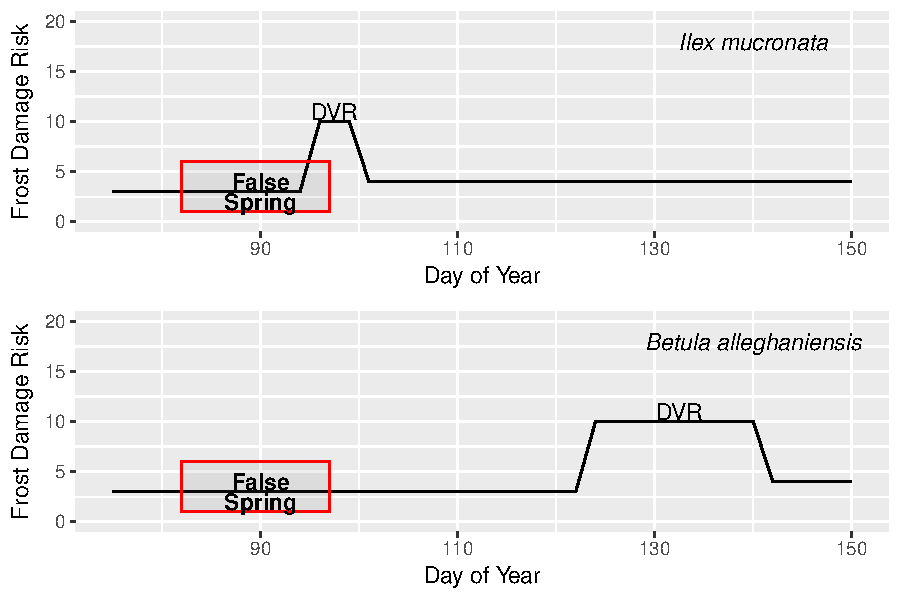
\includegraphics[width=\maxwidth]{figure/risk-1} 

}

\caption{A figure showing the differences in spring phenology and false spring risk across two species: \textit{Ilex mucronata} (L.) and \textit{Betula alleghaniensis} (Marsh.). We mapped a possible false spring event based on historic weather data and compared it to the observational data collected at Harvard Forest (O'Keefe, 2014). In this scenario, the \textit{Ilex mucronata} would be exposed to a false spring event, whereas the \textit{Betula alleghaniensis} would avoid it entirely. DVR stands for Duration of Vegetative Risk.}\label{fig:risk}
\end{figure}



\begin{figure} [H] 
 -\begin{center}
 -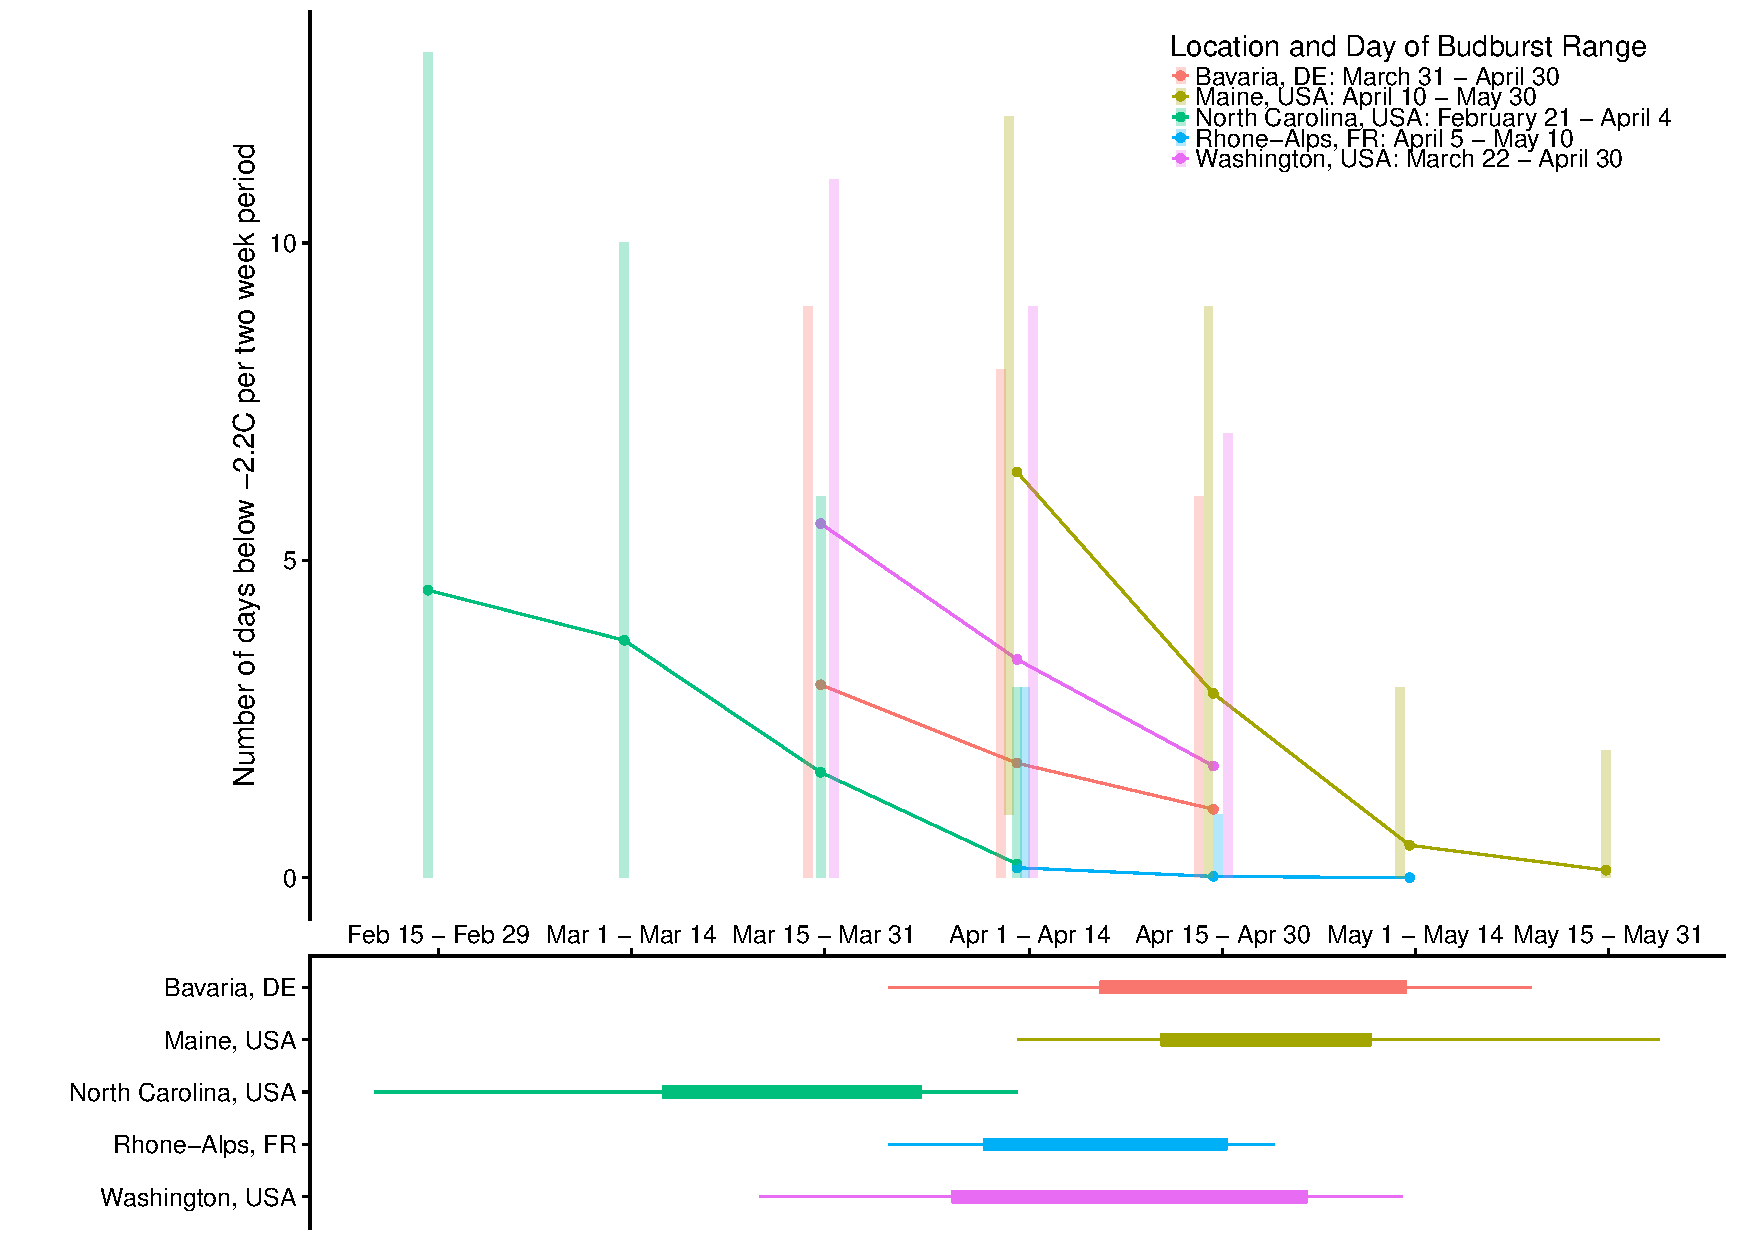
\includegraphics[width=16cm, height=13cm]{..//figure/RegRisk_clean.pdf} 
 -\caption{A comparison of false spring risk across five climate regions. By determining the average time of budburst to leafout dates for the dominant species in five archetypal climate regions, we were able to estimate the current spatial variation of false spring risk. We assessed the number of freeze days (-2.2$^{\circ}$C) (Schwartz, 1993) that occurred on average over the past 50 years within the average durations of vegetative risk for each region (USA-NPN, 2016; Soudani \textit{et al.}, 2012; White \textit{et al.}, 2009; Schaber \& Badeck, 2005).}\label{fig:regional} 
 -\end{center}
 -\end{figure}

\begin{figure}[H]

{\centering 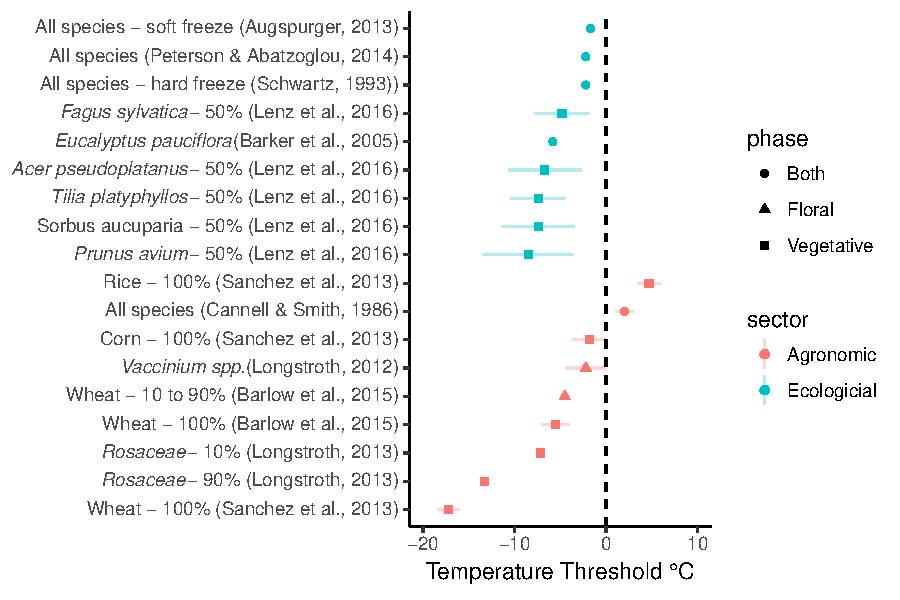
\includegraphics[width=\maxwidth]{figure/temp-1} 

}

\caption[A comparison of damaging spring freezing temperature thresholds across ecological and agronomic studies]{A comparison of damaging spring freezing temperature thresholds across ecological and agronomic studies. Each study is listed on the y axis along with the taxonimic group of focus. Next to the species name is the freezing definition used within that study (e.g. 100\% is 100\% lethality). Each point is the best estimate recorded for the temperature threshold with standard deviation if indicated in the study. The shape of the point represents the phenophases of interest and the colors indicate the type of study (i.e. agronomic or ecological).}\label{fig:temp}
\end{figure}


 
\begin{figure}[H]

{\centering 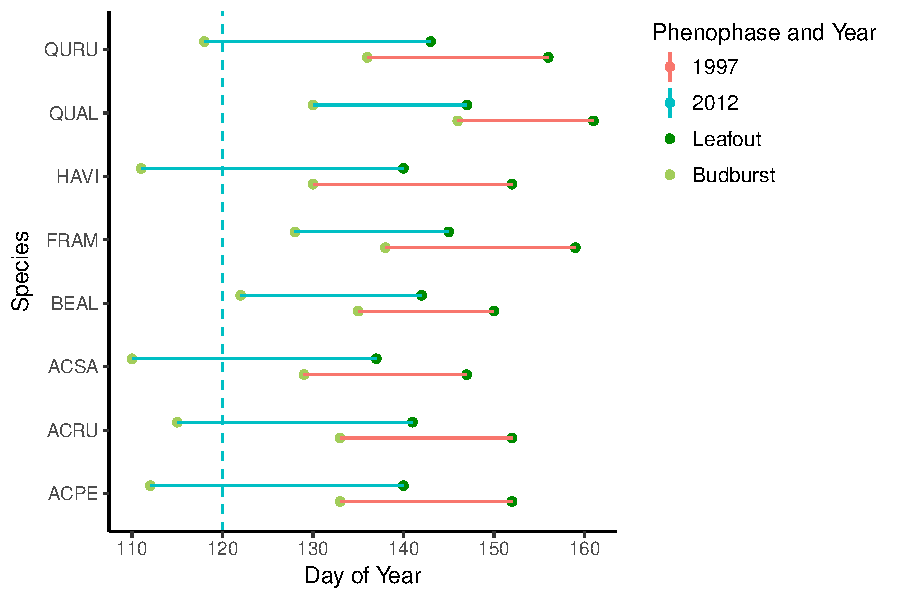
\includegraphics[width=\maxwidth]{figure/hf-1} 

}

\caption[Duration of vegetative risk for 8 species at Harvard Forest, comparing 1997 and 2012]{Duration of vegetative risk for 8 species at Harvard Forest, comparing 1997 and 2012. In 1997, the aggregated GDDs to budburst were the lowest and the durations of vegetative risk overall were shorter, whereas in 2012, the aggregated GDDs to budburst were the highest and the durations of vegetative risk were longer. The dotted line indicates a false spring event in 2012. The histogram at the bottom right corner indicates the frequency of accumulated GDDs to budburst for each year and indicates that 1997 was a thermally late year and 2012 was a thermally early year. }\label{fig:hf}
\end{figure}



\begin{figure} [H] 
 -\begin{center}
 -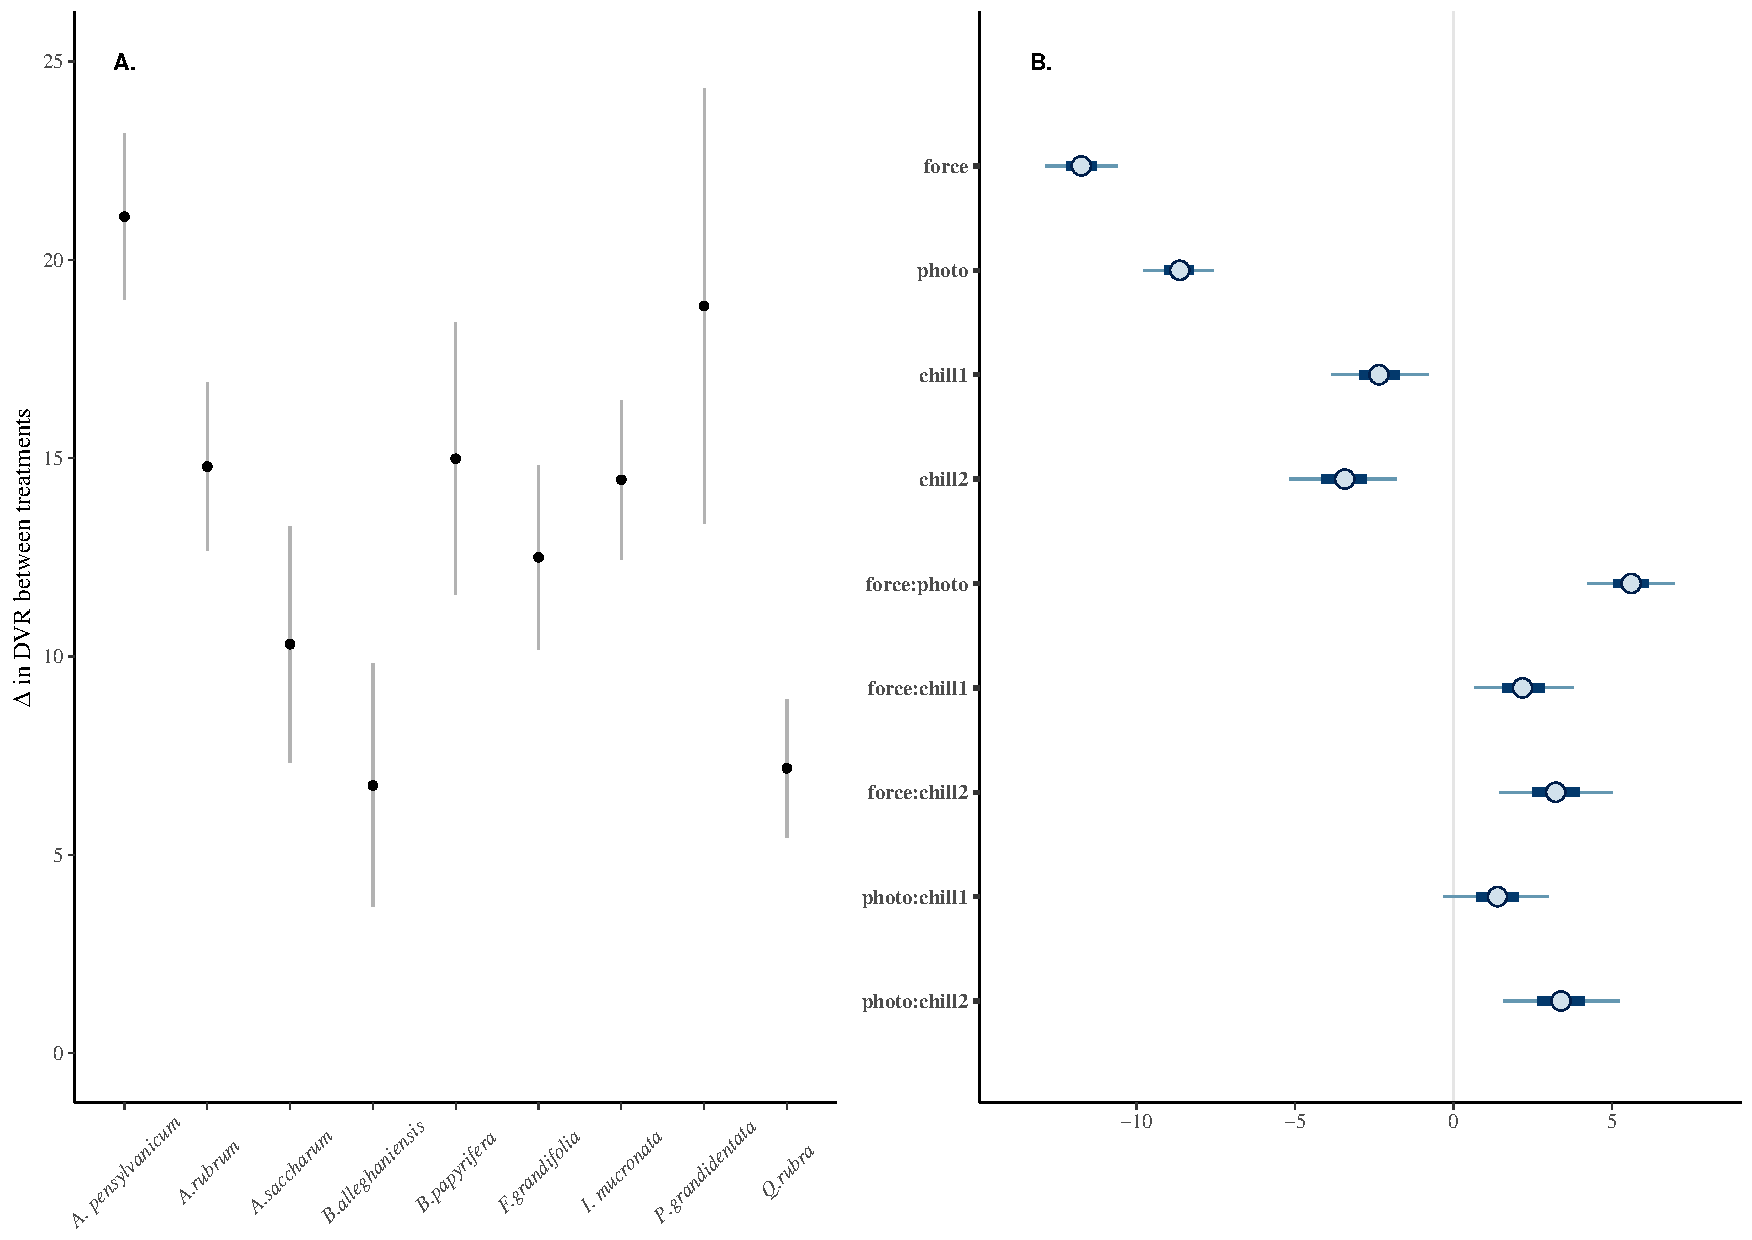
\includegraphics[width=16cm, height=13cm]{..//figure/DVRdiff_twoplots.pdf} 
 -\caption{Results from the growth chamber experiment. (A) Is a comparison of the durations of vegetative risk across two treatments for each species collected for the experiment. Species along the x-axis are ordered by day of budburst. Data was collected from a growth chamber experiment where one treatment had no additional overwinter chilling, low spring forcing temperatures, and shorter spring daylengths and the other had additional overwinter chilling, high spring forcing temperatures, and longer spring daylenghts. The standard error is represented by the bars around each point. (B) A plot of the parameter effects on the duration of vegetative risk. Spring forcing temperatures had the largest effect on the rate of leafout, with photoperiod also being a critical factor. However, they were offset by the interactions, especially the forcing and photoperiod interaction.}\label{fig:dan} 
 -\end{center}
 -\end{figure}

\nocite{Soudani2012}
\nocite{White2009}
\nocite{Schaber2005}
\nocite{Schwartz1993}
\nocite{Barker2005}
\nocite{Sanchez2013}
\nocite{Longstroth2012}
\nocite{Barlow2015}
\nocite{Longstroth2013}
\bibliography{..//refs/SpringFreeze.bib}

\end{document}
